% Preamble: \usepackage{graphicx,pdflscape,caption,geometry}
% Preamble: \DeclareCaptionFont{dppnine}{\fontsize{9}{11}\selectfont}
% The figure is native vector PDF, 770 x 480 PDF points.
% To retain the intended minimum 9 pt labels, do not downscale below 770 bp.
% A4 landscape with approximately 12 mm side margins accommodates 770 bp.
% For a journal with a smaller image area, re-layout the source; do not shrink.
% Replace the file path with the actual relative path in the LaTeX project.

\clearpage
\newgeometry{left=12mm,right=12mm,top=12mm,bottom=12mm}
\begin{landscape}
\begin{figure}[p]
  \centering
  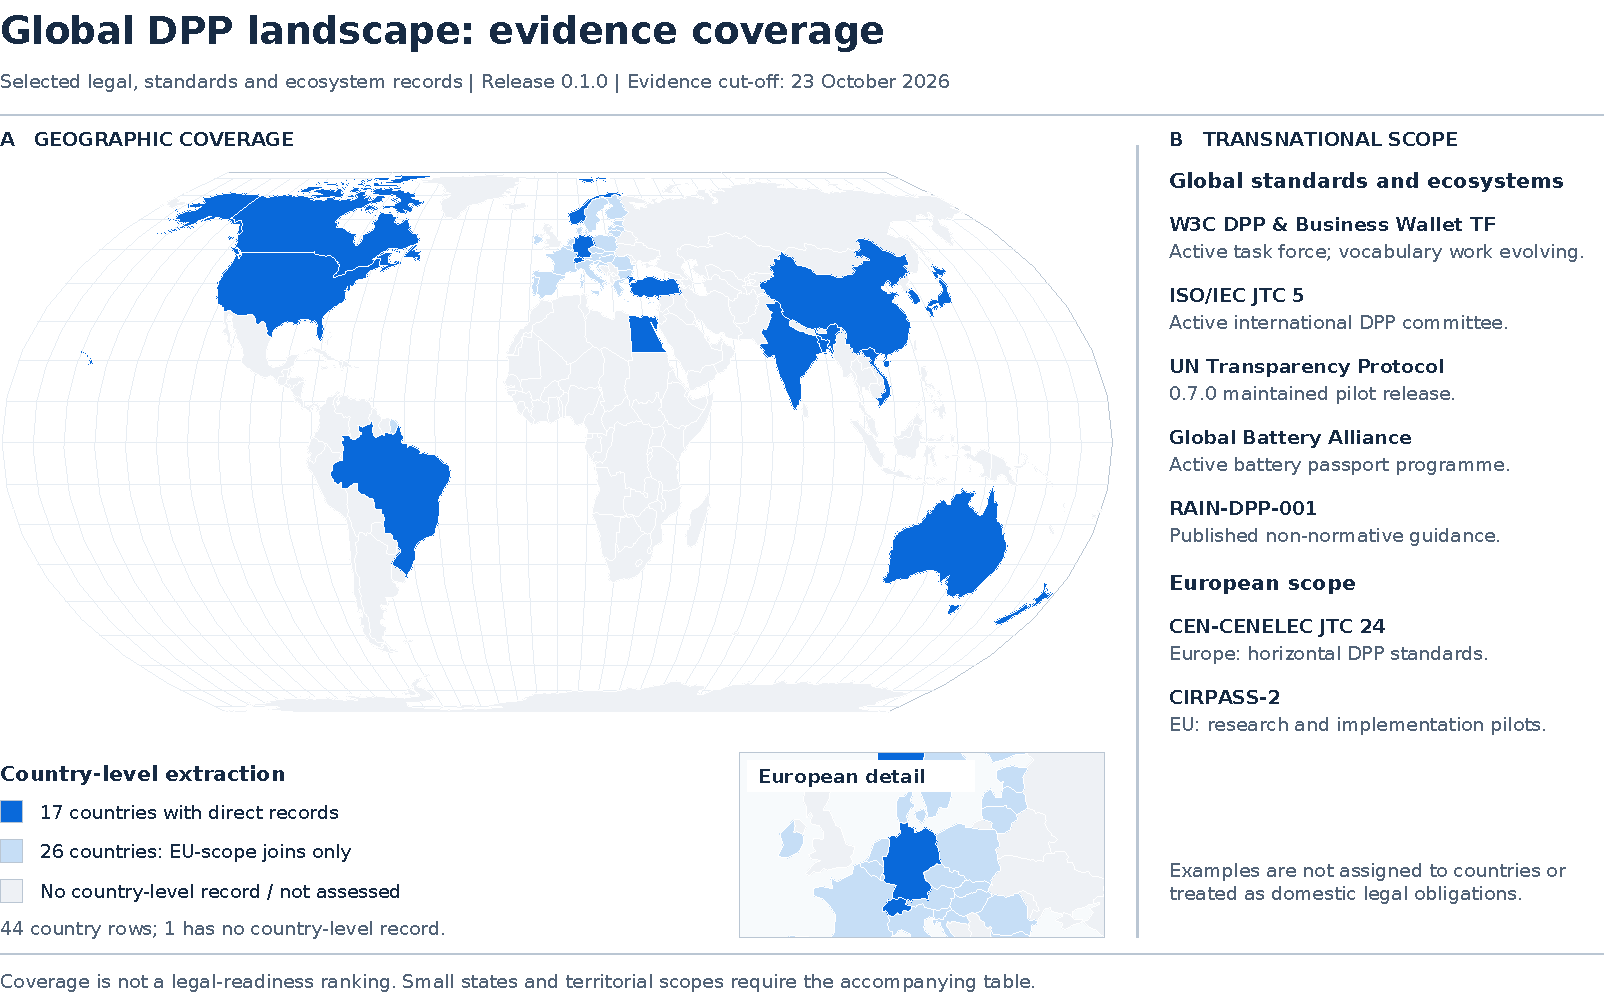
\includegraphics[width=770bp]{figures/landscape-world-map/dpp-world-map.pdf}
  \captionsetup{font=dppnine,skip=4pt}
  \caption{Selected DPP evidence coverage, release 0.1.0, 23 October 2026.
  Of 44 country rows, 42 have geometry; Malta and Singapore remain in the
  accompanying table. UK data has separate Great Britain and Northern Ireland
  scopes. Direct records and EU display joins do not establish national legal
  readiness; grey never means absence of law. Panel B shows transnational
  examples, not interoperability results. Sources: frozen release and
  Natural Earth v5.1.2. Human review pending.}
  \label{fig:global-dpp-coverage}
\end{figure}
\end{landscape}
\clearpage
\restoregeometry

% Add the full methodological qualifications from caption.md to the text or
% supplement. Add the release's durable citation/DOI once one actually exists.
% This snippet is an integration fragment, not a standalone compiled manuscript.
